\documentclass{article}

%............Inicia Preambulo.......................
\usepackage{graphicx}
\usepackage{float}
\usepackage[utf8]{inputenc}
\usepackage[shortlabels]{enumitem}
\usepackage{textcomp}
\usepackage{multicol}
\usepackage{caption}
\usepackage[spanish]{babel}
\usepackage[total={17.5cm, 23cm}, top=2cm, left=2cm]{geometry}
\usepackage{esvect}
\usepackage[font=footnotesize]{caption}

\spanishdecimal{.}
\parindent 0cm

%.............Fin de Preambulo........................

\begin{document}

\begin{center}
{\Large \textbf{Universidad Autónoma de Coahuila}}
\end{center}

\begin{center}
{\large Facultad de Ciencias Físico-Matemáticas}
\end{center}

%Materia
\begin{center}
{\large Metodos Numericos}
\end{center}

%Título
\begin{center}
{\large Newton-Rapson}
\end{center}

%Fecha
\begin{center}
{\large 29 de Noviembre del 2019}
\end{center}

%Autor
\begin{center}
{\large José Antonio Olveda García}
\end{center}

\vspace{5mm}

\begin{multicols}{2}

\section{Objetivo}
\label{sec:obj}
Analizar el metodo de buscador de raices por medio de Newton-Rapson, asi como ver las ventajas y desventajas que este programa pueda presentar.

\section{Introduccion}
\label{sec:Intro}


\section{Introducción}
\label{sec:intro}
Este método es uno de los mas utilizados para localizar raíces ya que en general es muy eficiente y siempre converge para una función polinomial.
\\
Se requiere que las funciones sean diferenciables, y por tanto, continuas, para poder aplicar este método.
\\
Se debe partir de  un valor inicial para la raíz: $x^{i}$ , este puede ser cualquier valor, el método convergirá a la raíz mas cercana.
\\
Si se extiende una tangente desde el punto$ [x_{i} ,f(x_{i})]$ el punto donde esta tangente cruza al eje x representa una aproximación mejorada de la raíz.
\\
La fórmula de Newton-Raphson se deduce a partir de la fórmula de la pendiente de una recta.
\\
Pendiente de una recta:

\begin{equation}
m=\frac{f(x_{2})-fx_{1}}{x_{2}-x_{1}}
\end{equation}

\begin{center}
$m=\frac{f(x_{i+1})-fx_{i}}{x_{i+1}-x_{i}}$
\end{center}

\begin{center}
$m=\frac{0-fx_{i}}{x_{i+1}-x_{i}}$
\end{center}

\begin{center}
$m (x_{i+1}-x_{i})=-fx_{i}$
\end{center}

\begin{center}
$x_{i+1}-x_{i}=-\frac{fx_{i}}{m}$
\end{center}

\begin{equation}
x_{i+1}=x_{i}-\frac{fx_{i}}{m}
\end{equation}

\begin{figure}[H]
\centering
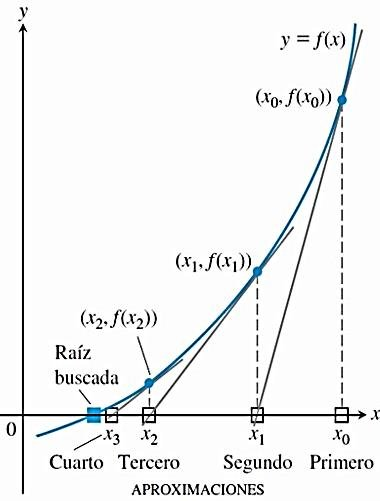
\includegraphics[scale=.5]{Newton-Rapson}
\caption{Grafica del metodo de Newton-Rapson}
\end{figure}

Se define la derivada de una funcion en un punto dado como la pendiente a la recta tangente de dicho punto, por lo tanto

\begin{center}
$m=f'(x)$
\end{center}
Hay que determinar un numero máximo de iteraciones

Normalmente esto se hace considerando una “tolerancia” , esto es:

El valor absoluto de la diferencia de la $x_{i+1}-x_{i}$ debe ser menor que la tolerancia o el resultado de alguna fórmula de error debe ser menor que la tolerancia dada.

Una de las fórmulas de error mas útiles es la del error relativo porcentual aproximado:

\begin{equation}
E_{a}=|\frac{X_{nueva}-X_{anterior}}{X_{Nueva}}|*100%
\end{equation}

El método de Newton-Raphson es convergente cuadráticamente, es decir, el error es aproximadamente al cuadrado del error anterior.

Esto significa que el numero de cifras decimales correctas se duplica aproximadamente en cada interacción.

Cuando el método de Newton-Raphson converge, se obtienen resultados en relativamente pocas interacciones, ya que para raíces no repetidas este método converge con orden 2 y el error $E_{i+1}$ es proporcional al cuadrado del resultado anterior $E_{i}$

Supóngase que el error en una iteración es $10^{-n}$ el error en la siguiente, (que es proporcional al cuadrado del  error anterior) es entonces aproximadamente $10^{-2n}$, el que sigue será aproximadamente $10^{-4n}$ etc.

De esto puede afirmarse que de cada iteración duplica aproximadamente el numero de dígitos correctos.

Sin embargo el método de Newton-Raphson algunas veces no converge, sino que oscila. Esto ocurre si no hay raíz real, si la raíz es un punto de inflexión o si el valor inicial esta muy alejado de la raíz buscada  y alguna otra parte de la función “atrapa” la iteración.

\section{Ejemplo}
\label{sec:Ejem}
Usa el metodo de Newton para estimar las soluciones de la ecuacion $x^{2}+x-1=0$. Empieza con $x_{0}=-1$ para la solucion de la izquierda, con $x_{0}=1$ para la solucion de la derecha. Despues halla $x_{2}$ para cada caso.

\begin{center}
$x_{i+1}=x_{i}-\frac{fx_{i}}{f'(x_{i})}$
\end{center}

\begin{center}
$x_{1}=x_{0}-\frac{x^{2}_{0}+x_{0}-1}{2x_{0}+1}$
\end{center}

\begin{center}
$x_{1}=x_{0}-\frac{x^{2}_{0}+1}{2x_{0}+1}$
\end{center}

Por la izquierda
\begin{center}
$x_{1}=\frac{(-1)^{2}+1}{2(-1)+1} = -2$
\end{center}

\begin{center}
$x_{2}=\frac{(-2)^{2}+1}{2(-2)+1} = -1.67$
\end{center}

\begin{center}
$x_{3}=-1.62$
\end{center}
Por la derecha
\begin{center}
$x_{1}=\frac{(1)^{2}+1}{2(1)+1} = 0.67$
\end{center}

\begin{center}
$x_{2}=\frac{(0.67)^{2}+1}{2(0.67)+1} = 0.619$
\end{center}

\begin{center}
$x_{3}= 0.618$
\end{center}
\section{Ventajas y desventajas}
\textbf{Ventajas}
1.La idea geométrica detrás del metodo de Newton-Raphson es
hacer una aproximacion de la funcion por medio de la recta
tangente en el punto $(x_{0}, f (x_{0}))$ y ver donde tal recta corta el eje de las x; ese valor de x es la siguiente aproximacion.
\\
2. A diferencia del metodo de biseccion, no hay una medida de
en cuanto se mejora cada aproximacion.
\\
3. En general, es mas rapido que el metodo de biseccion cuando
parte de una buena aproximacion.
\\
\\
\textbf{Desventajas}
\\
1. Lenta convergencia debida a la naturaleza de una función en particular. 
\\
2. Cuando un punto de inflexión, f’’(x) = 0, ocurre en la vecindad de una raíz.
 \\ 
3. No existe un criterio general de convergencia. 
\\
4. Tener un valor suficientemente cercano a la raíz. 
\\
5. Apoyarse de herramientas gráficas. 
\\
6. Conocimiento del problema físico. 
\\
7. Evaluación de la derivada.

\section{Impĺementacion del programa}
\label{sec:Imp}
Haciendo uso del programa de newton-raphson en el ejemplo aplicado, podremos comprobar si este metodo es realmente funcionable, donde confirmamos la precision que obtiene dicho programa sobre este
\begin{figure}[H]
\centering
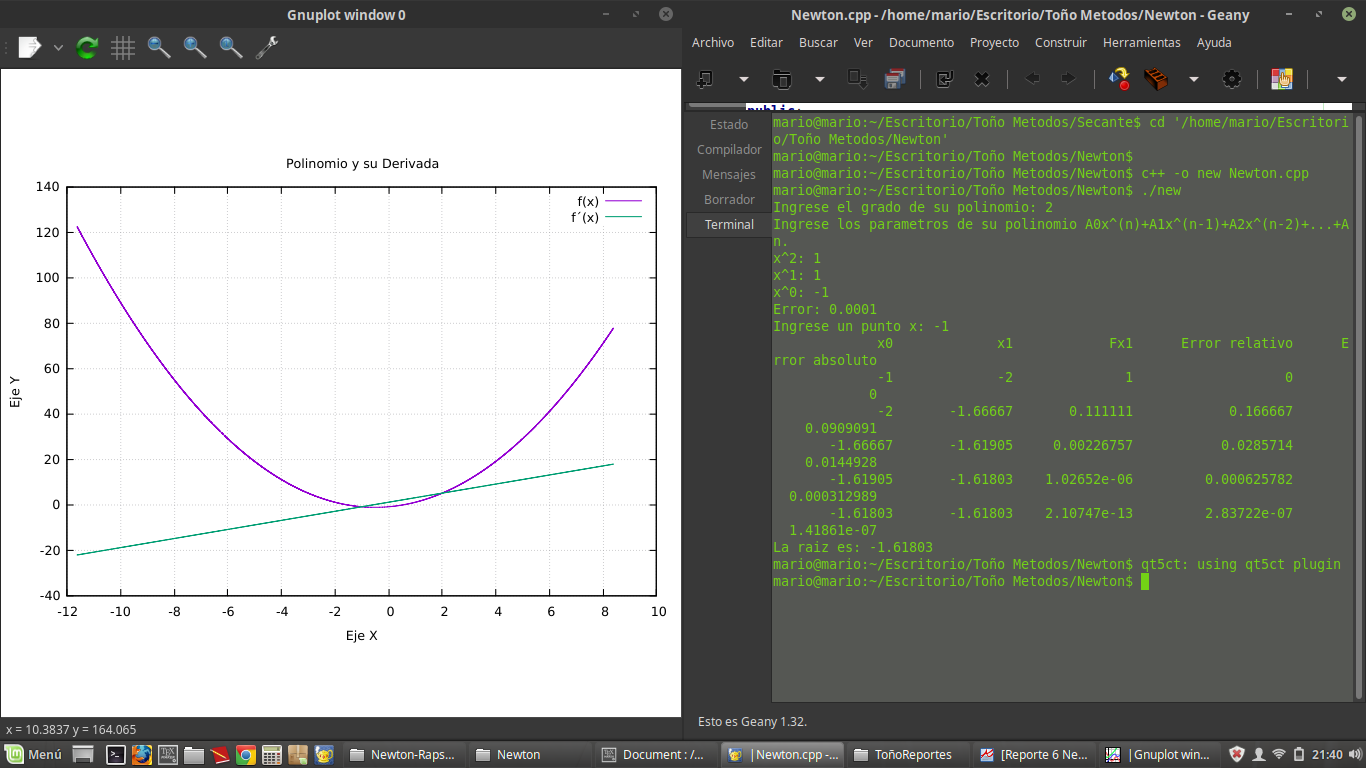
\includegraphics[scale=.125]{Newton-Raphson.png}
\caption{Programa de Newton-Raphson implementado como programa}
\end{figure} 
Como se logra apreciar en ambos casos del intervalo generado, se logra apreciar que las raices establecidas son correctas, sin embargo el programa presenta un mayor grado de aproximacion ante la grafica generada, asi como la graficacion de la funcion, esto con el objetivo de que el usuario pueda observar que es lo que esta sucediendo.


\end{multicols}

\end{document}